\documentclass[sigconf]{acmart}

\usepackage[english]{babel}
\usepackage{blindtext}

% Copyright
\renewcommand\footnotetextcopyrightpermission[1]{} % removes footnote with conference info
\setcopyright{none}
%\setcopyright{acmcopyright}
%\setcopyright{acmlicensed}
%\setcopyright{rightsretained}
%\setcopyright{usgov}
%\setcopyright{usgovmixed}
%\setcopyright{cagov}
%\setcopyright{cagovmixed}

\settopmatter{printacmref=false, printccs=false, printfolios=true}

% DOI
\acmDOI{}

% ISBN
\acmISBN{}

%Conference
%\acmConference[Submitted for review to SIGCOMM]{}
%\acmYear{2018}
%\copyrightyear{}

%% {} with no args suppresses printing of the price
\acmPrice{}


\begin{document}
\title{Exploring Feasibility of A Smart Robotic Wireless Access Point}

%\titlenote{Produces the permission block, and copyright information}
%\subtitle{Extended Abstract}

% \author{Paper \# XXX, XXX pages}
\author{Gabriel Righi \and Kendrit Tahiraj}
% \authornote{Note}
% \orcid{1234-5678-9012}
% \affiliation{%
%   \institution{Affiliation}
%   \streetaddress{Address}
%   \city{City} 
%   \state{State} 
%   \postcode{Zipcode}
% }
% \email{email@domain.com}

% The default list of authors is too long for headers}
\renewcommand{\shortauthors}{X.et al.}

\begin{abstract}
    The traditional consumer Wi-Fi setup involves a static access point, generally placed in the center of a home. As the number of internet connected devices have increased in homes, the demand for larger access point coverage has followed. Companies have invested in “mesh” network solutions, which are systems with multiple access points in the home, however these can be expensive and unpredictable. In this paper, we explore the feasibility of a smart robotic wireless access point that can follow your home’s traffic wherever it goes. We evaluated three distinct models for system operation (Roaming, Spinning, Save Points) using consumer-level products and firmware. Using the Save Points implementation, we successfully increased the received signal strength of a dynamically positioned client by 10 dBm in less than two (adjusted) minutes. Our evaluation of these implementations produced both successes and failures that should be used as a starting point for future research involving smart robotic wireless access points.
\end{abstract}

\maketitle

\section{Introduction}
The wave of a wireless signal is defined by three components: wavelength, wave speed, and frequency. In general, assuming the wave is traveling through air, wave speed will always be the speed of light. This leaves wavelength and frequency as the components of a wireless signal that can be controlled. There exists a tradeoff between these values, as they are inversely proportional to each other. Wireless signals with a longer wavelength travel further but have lower frequencies, while high frequency signals attenuate quickly. 

In wireless networking, this means that faster data transmission require a closer proximity and better line of sight. This tradeoff can be seen in many walks of life. A common example is 5G cell towers using mmWave technology. While mmWave enables data transmission at speeds far exceeding its mid- and low-band counterparts, it suffers from extreme attenuation \cite{mmWaveSurvey}. Even a hand obstructing the line of sight to a cell tower can significantly degrade the signal \cite{handBlock}. A similar distance tradeoff is seen in homes nationwide, where most consumer wireless routers support both 2.4GHz and 5GHz communication. The former of the two frequencies provides a larger range and deeper penetration but suffers in terms of speed when compared to the latter \cite{wirelessPenetration}. 

This tradeoff between signal strength and distance puts consumers in a no win-situation: Should they place their wireless access point (AP) in a central location to ensure broader coverage at the expense of faster 5GHz speeds, or position it closer to their primary workspace to take advantage of the high-frequency signal? While this choice might seem trivial, the difference is significant, as 5GHz signals can offer up to 10 times the data transmission rate when compared to their 2.4GHz counterparts. 

The prior situation highlights a less-discussed issue with APs. Most consumers place their AP in one location and never move it again. This static setup contrasts sharply with the dynamic nature of human activity, as people move around their homes throughout the day. It is easy to imagine scenarios where someone is at the furthest point in their house from the AP, experiencing poor signal quality simply because the AP is unable to adapt to their changing location.

This paper addresses the static AP issue with two primary aims. First, it proposes a solution: a dynamic wireless access point. Second, it evaluates various routing methods and their ability to maintain signal strength for users on the network. A dynamic AP solves the tradeoff between signal strength and signal speed by eliminating it almost entirely. By moving the AP to the user, the user can experience the best of both worlds: consistently fast speeds without needing to worry about connection strength. At its core, a dynamic AP requires two key components: a means of movement and a method to connect to users. For our tests, we utilized the iRobot Create 3 as the movement platform and the ASUS RT-AC86U as the consumer-grade AP. In lieu of access to a large home, all tests were run within the Thomas M. Siebel Center for Computer Science on the University of Illinois Urbana-Champaign campus. 

\section{Background}
\subsection{Received Signal Strength Indicator}
Received signal strength indicator (RSSI) is a measurement of the power level of a received radio signal. For wireless networking, RSSI is used for determining the strength of a signal between a client and an AP. Signals will attenuate naturally as they are sent through some medium. This attenuation means that when an AP receives a signal, the power of the original sent signal will be reduced by some amount based on how far that signal traveled. In general, a signal that is being sent from a closer position to the AP will have a larger RSSI than a signal sent from further away. Due to multipath and environmental factors, this may not always be the case, but it is often true.

\subsection{iRobot Create 3}
The iRobot Create 3 is a product derived from the popular Roomba vacuum. Built on the same platform, it mirrors the Roomba, but lacks vacuuming capabilities. For the purposes of this paper, the Robot is valued solely for its ability to move while carrying a load. Its movement options include rotating, moving forward or backward, and navigating based on an imaginary grid of points. The Robot does not feature built-in mapping or navigation capabilities. While external packages may provide advanced routing options, these are beyond the scope of this project.

\section{Related Work}
\subsection{RSSI Localization}
The most common form of localization is the Global Positioning System (GPS). While GPS is highly accurate outdoors due to its usage of satellites, it performs far worse indoors. GPS signals are prone to interference and are often too weak to penetrate indoor spaces.  This has led to research involving using RSSI as a method of indoor localization. In wireless communication, RSSI can be used as a measure of distance between devices based on signal strength. With 3 APs measuring the RSSI of the same device, trilateration can be employed to estimate the true location of the device rather than just the distance \cite{rssiLocalization}.

Trilateration works as follows: Each AP calculates its distance to the client device based on RSSI. Then each AP will draw a circle around itself, with the radius representing the measured distance. The intersection points of the circles drawn by each AP represent potential positions for the client. The only necessary information for this calculation is the RSSI and the real-world position of the APs. RSSI localization is effective when up close (less than 5 meters), but as the distance increases it becomes far less accurate. 

\begin{figure*}[tp]
\centering
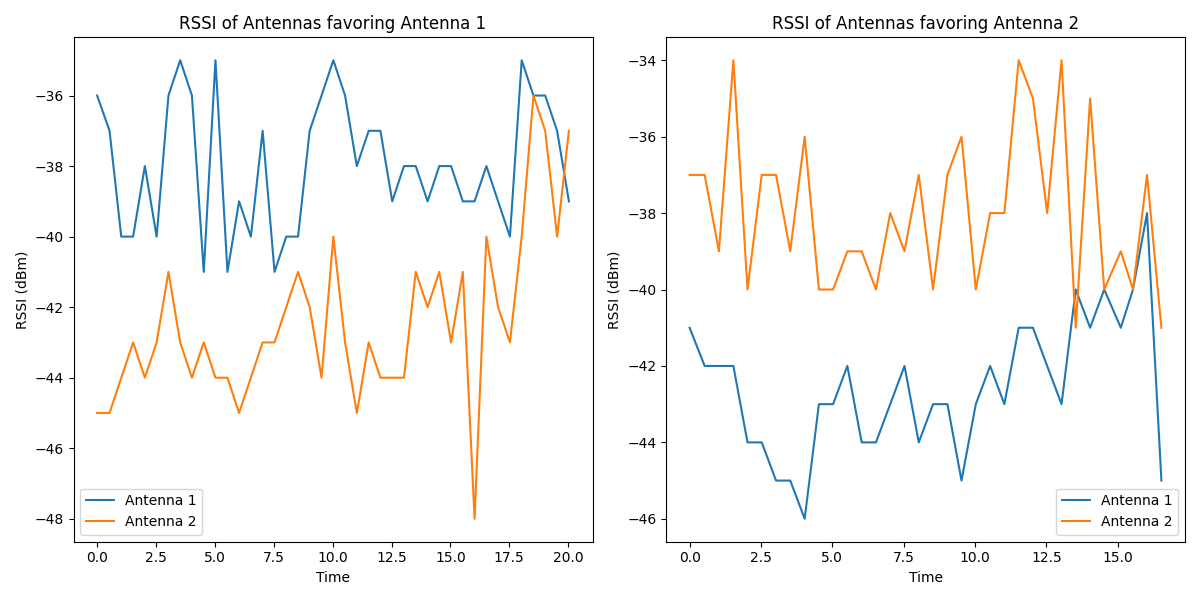
\includegraphics[width=\textwidth]{figures/antennas_comparison}
\caption{RSSI of AP when client position favors one antenna.}
\label{fig:antennas_comparison}
\end{figure*}

\section{System Design}
The optimal routing method for our dynamic access point is not immediately clear. Therefore, this paper introduces three distinct methods to comprehensively evaluate the potential of a robotic access point.

\subsection{Roaming}
The roaming method is an intuitive approach to routing with an indicator like RSSI. The idea is to “roam” towards directions to find the location of optimal RSSI in a home. The robot starts by roaming around its starting point at random. If the RSSI has increased a favorable amount while moving in a given direction, the robot sets its new starting point to its current location and begins roaming once again. Since the robot is continually moving to higher RSSIs, it follows it should eventually converge to a location with an RSSI above a desired threshold. Once it reaches this it will wait until quality worsens, where it will then repeat the process.\par

Roaming has the benefit of, navigation aside, being dynamic to any environment with little user configuration. It could theoretically follow a user wherever they go and could be programmed to safely navigate the environment rather than move randomly, though this is not trivial.

\subsection{Spinning}
The goal of the spinning method is to narrow down the general direction of the client and intelligently move in that direction until a goal RSSI is achieved. Upon worsening, the method should wake and repeat. This method requires attaching two antennas to the top of the robot. We use this setup to get the location of the client by comparing the per antenna RSSI every X degrees (30 by default). If the ratio of \(\frac{a1}{a2}\) or \(\frac{a2}{a1}\) is larger than a threshold value (1.1 by default), we use that as our direction and move towards it for a distance before repeating all the steps. This should eventually converge to a location that can achieve some desired RSSI value.

Like Roaming, assuming navigation can be handled smoothly, this solution is dynamic to any environment and has no implied user configuration. Since this method calculates before moving rather than constantly guessing, it should result in a higher movement efficiency. This comes at the cost of a higher calculation overhead (as sampling RSSI and rotating the robot takes time).

\subsection{Save Points}
Save Points looks to take advantage of household habits by having an internal mapping of preferred spots around the house instead of being fully dynamic. The robot should linger at one of these positions if the RSSI is under a desired threshold, and should continue to recalculate it’s RSSI while it is physically idle. Once the connection worsens, the robot should route to its other “save points” in sequence until the goal RSSI is seen again. If the goal RSSI is not found, it will continue to roam until it is. 

This method relies less on localization and features more predictable movement, which is preferred in this case to reduce the risk of the robot becoming a tripping hazard by stopping frequently in the middle of rooms or hallways. Save points allow the user to designate specific locations, such as room corners or other expected areas for the robot. The downside to save points is it does require the user to use the internet somewhere near one of the points, and knowing where to put the points  also requires the user to have some idea of where they most commonly use the internet.

\section{Results/Validation}
In evaluating how well the proposed methods function, we will be measuring 2 factors. The first factor is RSSI. As mentioned in the introduction, the primary goal of this project is to ensure strong WiFi signal strength from any location within a home. If the RSSI between the client and the AP converges to a higher value, it indicates that the movement method effectively strengthens the client’s connection. The second factor measured is time to converge. If the RSSI does converge but it takes hours to do so, it will not be useful in real world situations. The movement methods should converge within minutes of the user moving to a new location, barring extreme movement by the client. 

For our tests, we will position the robot approximately 15 meters away from the client. Each method will give the robot around 2 minutes of adjusted time to optimize its RSSI. Due to significant latency occasionally introduced by our Bluetooth connection when sending commands, we adjust the timing. Whenever we refer to "adjusted time," it indicates the period during which the robot has actively started or completed executing a command.
\subsection{Roaming}

\begin{figure}[tp]
\centering
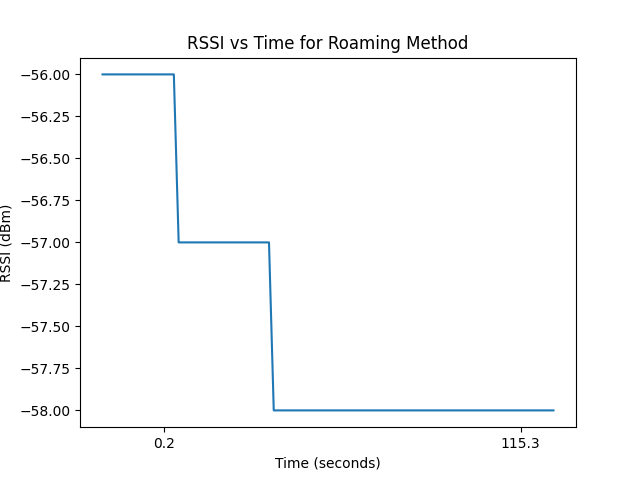
\includegraphics[scale=0.5]{figures/rssi_roaming}
\caption{RSSI of the Robot as it attempts to increase signal strength via the Roaming method. }
\label{fig:rssi_roaming}
\end{figure}

While roaming may seem like an effective approach for lowering the RSSI quickly, in application, it does quite the opposite. During our trials, we observed that the RSSI of the robot did not consistently improve, and its movement often resulted in reduced connection quality. Throughout our tests, we manipulated various factors in an effort to enhance roaming effectiveness, primarily adjusting the distance the robot traveled before re-averaging the RSSI. Despite changing the roaming parameters, the method itself proved ineffective. This can be seen in Figure~\ref{fig:rssi_roaming} which is demonstrative of the results of our trials. The RSSI got worse over the 2 minute trial and had no clear convergence. 

When thinking about why roaming doesn’t work as a solution, we must revisit how RSSI works. RSSI performs best within a 5 meter radius, where changes in signal strength are most noticeable. In our tests, with the robot ~15 meters from the AP, the RSSI changes from the robot did not consistently register as smaller when moving towards the router. Our tests tried movement distances up to 3 meters without registering a consistent change in RSSI. A greater movement distance than this would likely be necessary for the Robot to register a consistent change. This is not really feasible, as the robot could potentially move very far away from the router, causing a signal drop, or it would be unable to move such a great distance easily, as it must navigate through a house and cannot move in straight lines.
\subsection{Spinning}
\begin{figure}[tp]
\centering
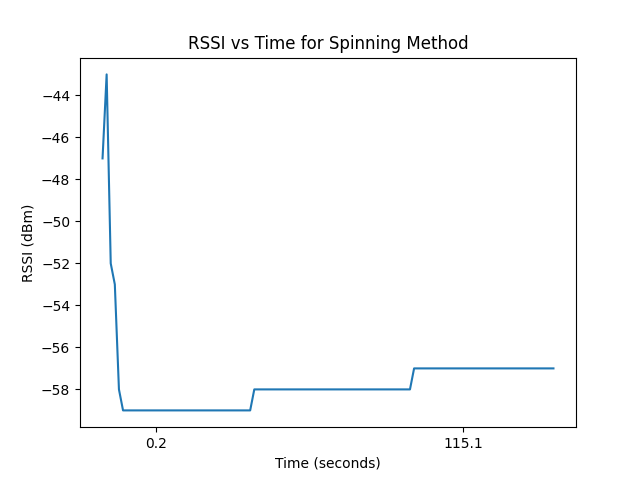
\includegraphics[scale=0.5]{figures/rssi_microwave}
\caption{RSSI of the Robot as it attempts to increase signal strength via the Spinning method.}
\label{fig:rssi_microwave}
\end{figure}
Aligning the antennas such that the difference in signal strength is maximized does work in theory but falls flat in practice. As shown in Figure~\ref{fig:rssi_microwave}, there is no clear improvement in RSSI, and much like with roaming, the RSSI got worse over the majority of our trials. While the robot would sometimes move in the correct direction, this was never consistently the case. 

The issue with the spinning method is the antennas are not far enough apart to have a noticeable RSSI change between them. As stated earlier, RSSI changes are most noticeable within 5 meters, and when both antenna are ~15 meters away, RSSI is just not consistent enough for the difference in the antenna strengths to be significant. One could imagine a massive contraption that would place the antennas meters away from each other, but that would not be practical as it would drastically increase the floor profile of the robot. 
\subsection{Save Points}
\begin{figure}[tp]
\centering
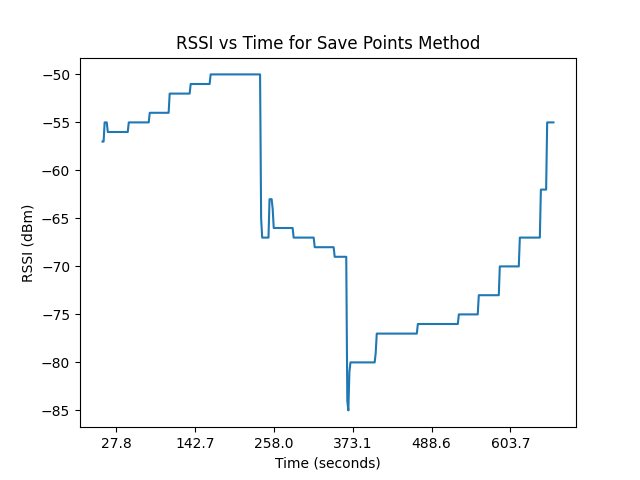
\includegraphics[scale=0.5]{figures/rssi_save_points}
\caption{RSSI of the Robot as it attempts to increase signal strength via the Save points method.}
\label{fig:rssi_save_points}
\end{figure}
Save points is the only algorithm we tested that consistently had successful results. During our tests, when we placed the client near a save point, the robot would route to the nearest point and wait there until we moved the client to a new position.  The robot converged in < 2 adjusted minutes every time we positioned the client near a save point. This is illustrated in Figure~\ref{fig:rssi_save_points}, where the RSSI stabilizes around 200 seconds and 650 seconds. At these points, the robot stopped because the RSSI exceeded the threshold for a strong connection, and we verified that it was positioned at the expected save point near the client.

Save points works well because it offers a structured roaming approach. By moving between save points that are placed apart at larger distances, the problem of RSSI not significantly changing is avoided. This approach also avoids complex routing issues since the robot follows the points like a grid, and a path can be easily defined via the grid. An observed downside of save points is that the robot could still path out of range of the router. This could be mitigated with a more intelligent approach that stops pathing in a direction once the RSSI becomes bad enough.

\section{Conclusion}
Many of the failures recorded in our experiments were due to the inaccuracy and unpredictability of RSSI. From this we have concluded that an optimal smart robotic AP should not focus on optimizing RSSI during random movement, but rather focus on RSSI upon predefined paths. Building on this idea, we determined that the "Save Points" approach was the most effective and pragmatic implementation of a dynamic AP. Letting the user configure where the robot will frequent can limit the robot’s search space significantly, providing better efficiency and a greater real-world experience overall. We predict that other solutions may come to the same conclusion, and the focus will shift to making the intermediate movement more efficient to squeeze the most performance out of multiple preferred AP positions. We also look forward to seeing further research using lower-level channel state information (CSI) to have a more reliable indication of where client devices are, instead of solely relying on RSSI.


\bibliographystyle{ACM-Reference-Format}
\bibliography{reference}

\end{document}
